\section{Experimental Setup}

%%%%%%%%%%%%%%%%%%%%%%%%%%%%%%%%%%%%%%%%%%%%%%%%%%%%%%%%%%%%%%%%%%%%%%%%%%%%%%%%%%%%%%%%%%%%%%%%%%%%%%%%%%%%%%%
%Initiator: Ran Itay
%Last modified by: MM Devi, May 26 2017
%Comment: The detector section has been modified. MMdevi's changes are made in blue
%%%%%%%%%%%%%%%%%%%%%%%%%%%%%%%%%%%%%%%%%%%%%%%%%%%%%%%%%%%%%%%%%%%%%%%%%%%%%%%%%%%%%%%%%%%%%%%%%%%%%%%%%%%%%%%

In order to identify \superradiance\ effects in LXe, the temporal and spatial properties of scintillation events should be studied and quantified. In the \direxeno system LXe is circulated through a small spherical cavity held in a thick sphere made of high purity fused silica (HPFS). The sphere is surrounded ($\sim4\pi$) by PMTs allowing high resolution, both spatial and temporal, measurements of individual photons. The PMTs do not come in contact with the xenon, so less impurities are introduced to it, and the material selection is less stringent. The geometrical design of the system approximates a point  source of scintillation photons, and a detailed vertex reconstruction within the LXe bubble is unnecessary. A schematic view of the system is shown in Fig~\ref{fig:detSch} . 

\begin{figure}[h]
\centerline{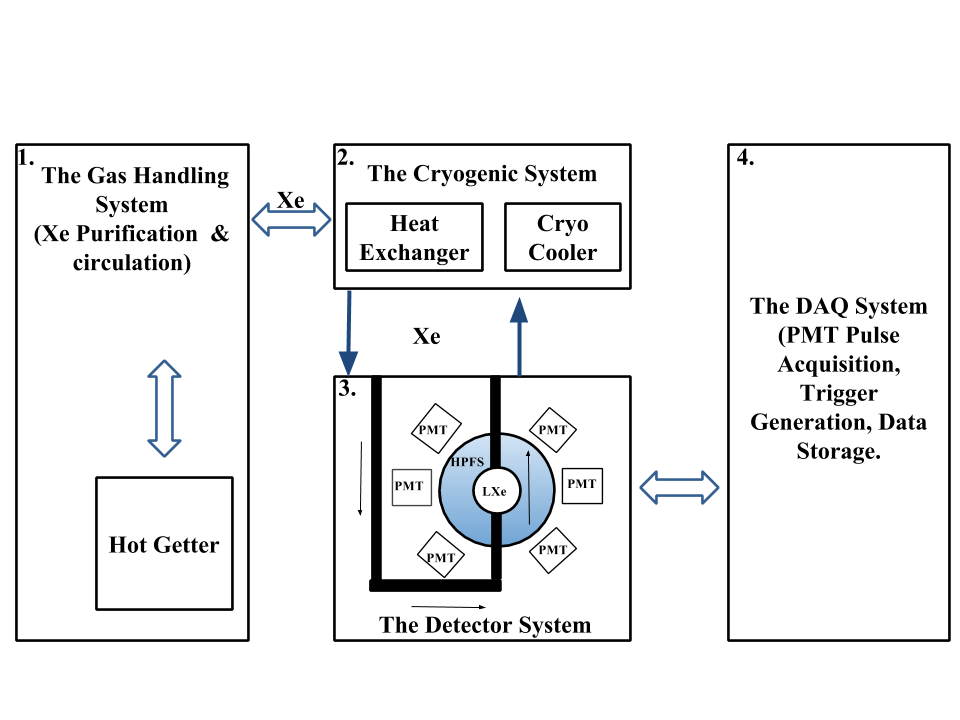
\includegraphics[width=0.8\linewidth]{DetSch.png}}
\caption{A schematic view of \direxeno.}
\label{fig:detSch}
\end{figure}


The current system is designed with $\sim1$\,ns time resolution, less than $1$\,ns synchronization between PMTs, and $\sim0.8$ radians spatial resolution. Since the exact nature and magnitude of \superradiance\ in LXe is yet unknown a guiding principle in the design was flexibility to upgrades or redesign of any part of the system to fulfill any future experiment requirements. The modular design allows fast and easy recovery in case of components malfunction.

The system is made of five main building blocks. (i) \textbf{The gas handling system} which in normal working mode circulates the xenon and purifies it. (ii) \textbf{The cryogenic system}, liquefies the xenon and 
delivers it to the detector system. (iii) \textbf{The detector system} consists of an HPFS sphere that holds a small bubble of LXe target, and PMTs around it. (iv) \textbf{The DAQ system} supplies High Voltage (HV) 
to the PMTs and handles triggering and digitization of data. (v) \textbf{The slow control (SC) system} monitors the condition of the experiment using various gauges and also sends alarms if some measurements exceed normal values. The entire assembly is held on 3 separate racks as shown in Fig.~\ref{fig:fulldet}.



\begin{figure}[h]
\centerline{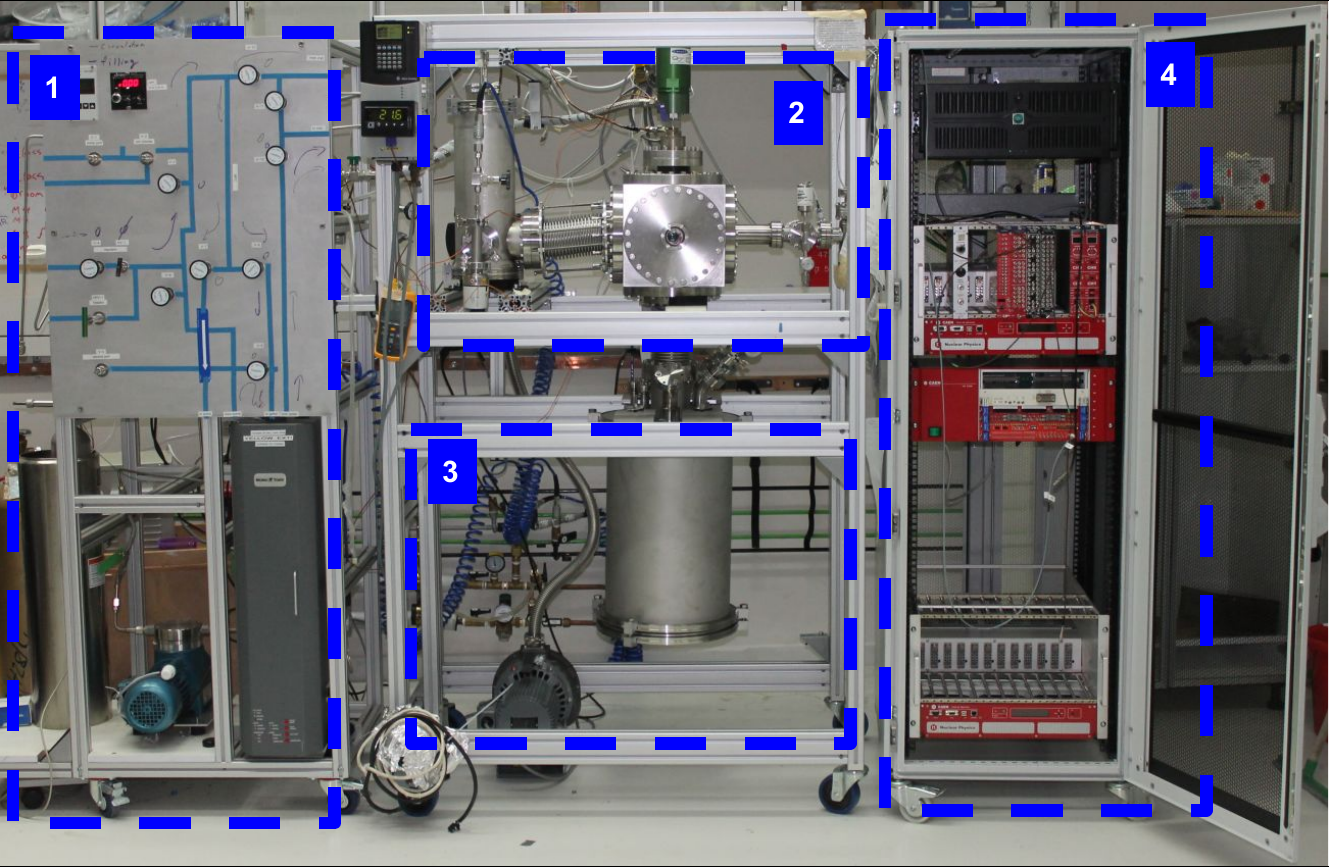
\includegraphics[width=0.8\linewidth]{FullSys.png}}
\caption{The \direxeno system mounted on the three racks. 1. The gas handling system. 2. The cryogenic system including the heat exchanger. 3. The detector chamber. 4. The Data acquisition system. The SC system is distributed around all 3 racks.
\label{fig:fulldet}}
\end{figure}



\subsection{The Gas Handling System}
\label{subsec:gas}

In \direxeno, only the prompt scintillation is measured, so a high level of LXe purity is not of a great importance. However in many LXe detectors the desired level of impurity concentration is at the level of 1\,ppb O$_2$ equivalent~\cite{Aprile:2009dv}, this is crucial to allow 
ionization electrons drift for several cm. To reach that purity level in a reasonable amount of time (several days instead of months), 
a continuous purification is needed. The gas handling system provides this process along 
with all gas handling operations such as filling, recuperation and circulation. The xenon circulation also plays a major role in heat transfer.


During purification, The xenon is forced by a circulation pump\footnote{N143 SN.12E AC 230V50HZ KNF diaphragm circulation pump} extracting LXe from the detector part through a heat exchanger\footnote{GEA GBS100M-24 plate heat exchanger},
where it is heated and vaporized, into a hot getter\footnote{MONO-TORR PS4-MT15-R-2} which cleans the xenon. The xenon passes through a mass flow controller\footnote{MKS mass flow controller 1179A00614CR1BM} (MFC), 
enabling monitoring and controlling the amount of heat introduced to the system.  Once purified, the xenon is delivered back to the cryogenic system 
via the heat exchanger, where the remaining GXe is 
liquefied before flowing back to the detector part. A schematic of this 
system is shown in fig.~\ref{fig:gasSchematic}.


%%%%%%%%%%%%%%%%%%%%%%%%%%%%%%%%%%%%%%%%%%%%%%%%%%%%%%%%%%%%%%%%%%%%%%%%%%%%%%%%%%
\begin{figure}[h]
\centerline{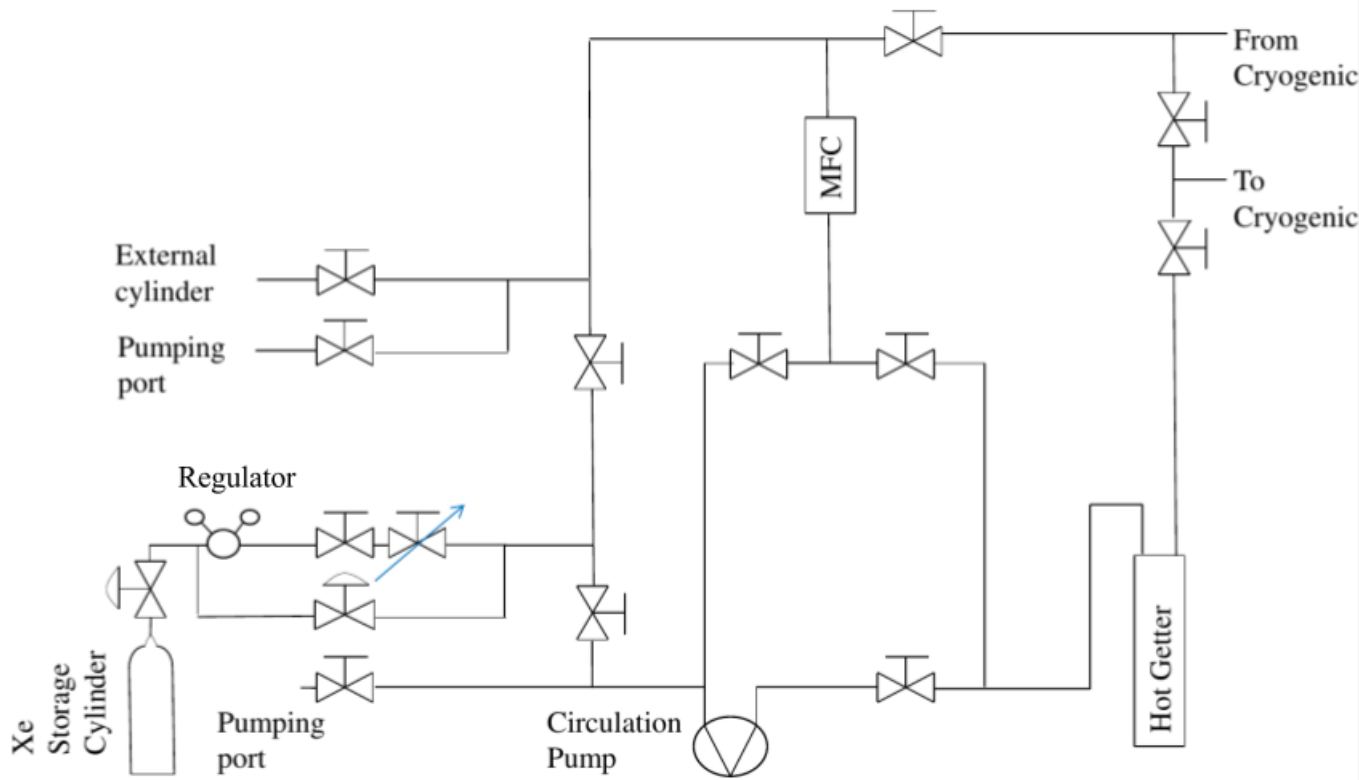
\includegraphics[width=0.75\linewidth]{GasSchematics.png}}
\caption{Schematics of the gas handling system. High pressure valves are indicated as 
valves with arcs. Needle valves are indicated as 
a valve with an arrow.
\label{fig:gasSchematic}}
\end{figure}
%%%%%%%%%%%%%%%%%%%%%%%%%%%%%%%%%%%%%%%%%%%%%%%%%%%%%%%%%%%%%%%%%%%%%%%%%%%%%%%%%%


\subsection{The Cryogenic System}
\label{subsec:cryo}

Remote cooling is generally used in LXe experiments due to reduction in background radiation and acoustic noise from the cooler to the detector, and due to design flexibility. The cryogenic system is connected to the gas handling system on 
one side and to the detector part on the other, and built such that replacing the cryo-cooler type (e.g., to PTR) requires just an adaptation to the top flange.


The cryogenic system is divided to an Outer Vessel (OV) which holds 
the insulation vacuum, and an Inner Vessel (IV) which holds the xenon. In addition to the vacuum which prevents heat leakage due to diffusion and convection, the IV is fully covered by multi layer Aluminized Myler to prevent heating via radiation.  

%%%%%%%%%%%%%%%%%%%%%%%%%%%%%%%%%%%%%%%%%%%%%%%%%%%%%%%%%%%%%%%
\begin{figure}[h]
\centering
\begin{subfigure}[c]{0.35\textheight}
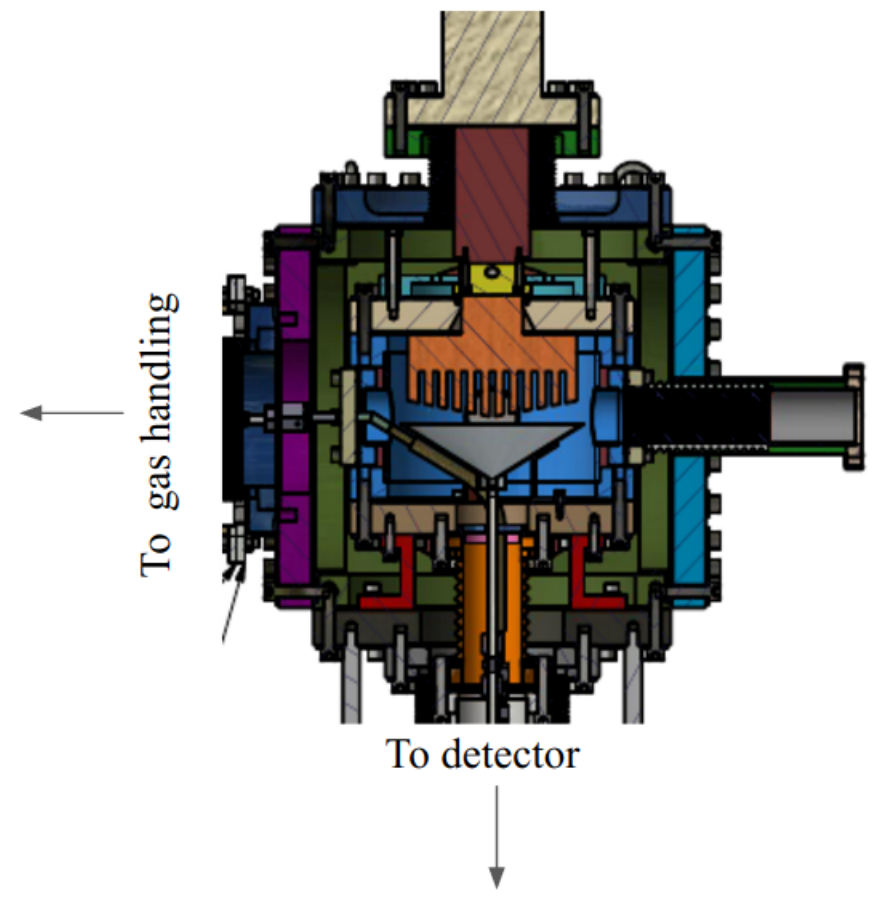
\includegraphics[width=\textwidth]{cryoMirror.png}
\end{subfigure}
\begin{subfigure}[c]{0.25\textheight}
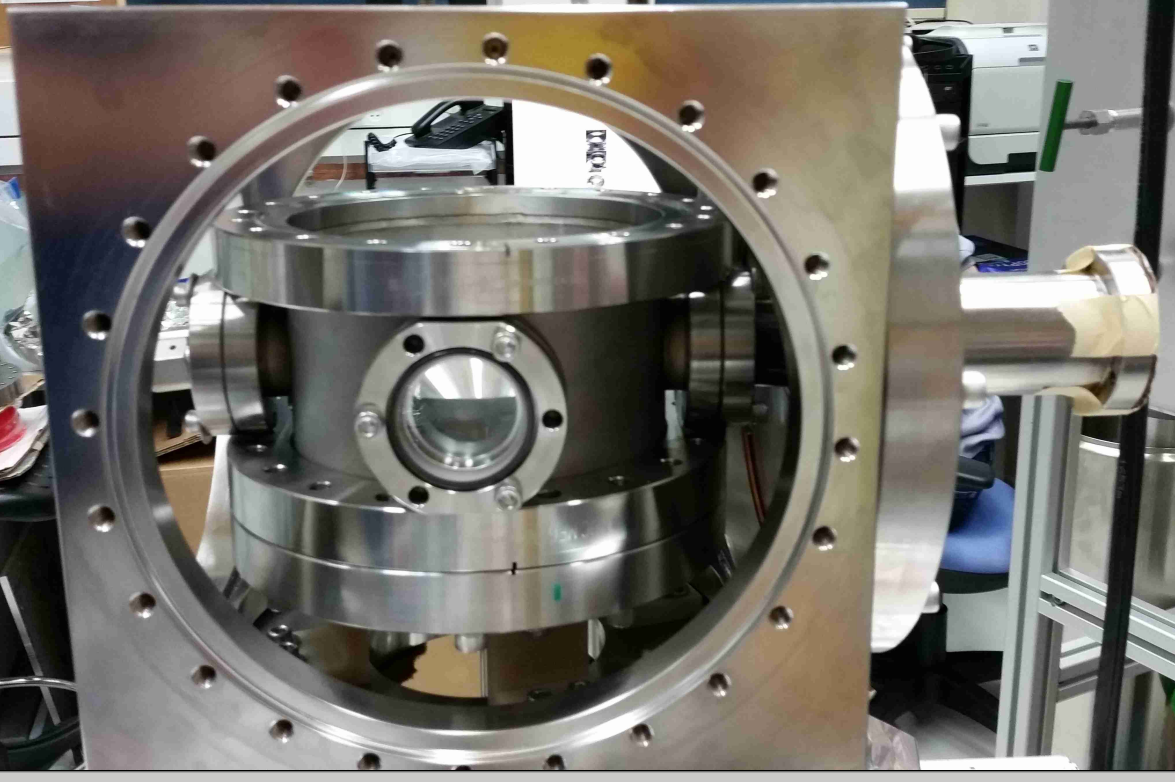
\includegraphics[width=\textwidth]{cryoOpenCrop.png}
\end{subfigure}
\caption{ CAD view of the cryogenic system(Left) and a picture of the cryogenic system (Right). 
\label{fig:cryo}}
\end{figure}
%%%%%%%%%%%%%%%%%%%%%%%%%%%%%%%%%%%%%%%%%%%%%%%%%%%%%%%%%%%%%%%%




The OV is made of a 10" Conflat (CF) cube, with ports on all six faces, interfacing the gas handling system and  the detector part, and bearing service ports (e.g., feed-throughs, pumping ports, 
view ports). The OV is connected to the detector part via a 6" CF flexible bellows, providing a shared vacuum space.

The IV is made of 1.5" long cylinder with 6" CF flanges on both sides, holding xenon within. A 120~\,mm diameter cold finger is welded to its top flange. The design of the cold finger is similar to the one in~\cite{xe100_instr2012}. The inner part of the cold finger is made of long fins, resulting in a better heat transport.  The upper part of the cold finger is in thermal contact with the 
QDrive cryo-cooler~\footnote{QDrive 20BB 9p6 A 3 AYNBNCO} via a copper adapter. The copper adapter 
holds two $100\Omega$ pt resistor\footnote{PT111 Lakeshore} which are connected to a PID reader\footnote{cryo-con model 
18i Cryogenic Temp Monitor} for temperature measurements. A cartridge-heater 
is also inserted to the copper adapter for emergency heating in case xenon freezes on the 
cold finger. 

The cryo-cooler is connected via a $4\sfrac{1}{2}$" 
flange to the OV top flange. While usually cryo-coolers used for 
xenon experiments constantly operate in maximal cooling, the QDrive cryo-cooler utilizes a 
temperature control to vary its cooling power up to $\sim$70\,W. This allows setting a desired working temperature which is constant within less then $0.1~\mathrm{^{\circ}C}$ measured on the cryo-cooler.

On the inner side of the IV bottom flange a thin 0.6~mm Stainless Steel (SS) funnel is installed 
collecting LXe drops from the cold finger, and delivering them to the  detector. This flange is attached to the detector part, via a $3\sfrac{3}{8}$" flexible bellows. The 
bellows hosts two pipes connected to the circulation system, and a third pipe coming 
from the funnel. The three pipes deliver LXe whereas the GXe is filling the bellows volume. The purer LXe (from the gas handling system) and the less pure LXe (from the cold finger) are separated, and can be delivered to different parts of the system. Some of the guidelines for the design of 
the cryogenic system are based on~\cite{Giboni}. The CAD view of 
the design of the cryogenic system and a photo of the actual system are shown in Fig~\ref{fig:cryo}. 

%%%%%%%%%%%%%%%%%%%%%%%%%%%%%%%%%%%%%%%%%%%%%%%%%%%%%%%%%%%%%%%%%%%%%%%%%%%%%%%%%%%%%%%%%%%%%%%%%%%%%%%%%%%%%%%%%%%%%%%%%%%%%%%%%%%%%%%%%%%%%%%%%%%%%%%%%%%%%
\subsection{The Detector System}
\label{subsec:det}
 
The detector system refers to a vacuum chamber and its inner assembly consisting of a transparent sphere that 
contains the LXe, the PMT sensors observing it and their accessories. This chamber is placed below the cryogenic system. 


The interface unit to the cryogenic system is built out of two flanges welded together via seven tubes, which serve as service ports for electrical and other feedthroughs: four with a $2 \sfrac{3}{4}$" CF flange, and three with a $1\sfrac{1}{3}$" CF flange (mini-CF). 
The upper flange, ISO-K NW320, shares the cryogenic system's OV insulation vacuum, while the bottom one, CF-10", is part of the IV and could hold xenon for future detectors. 
The CF flange is also adapted to fit a smaller CF-$4\sfrac{5}{8}$" flange which is currently used.

The vacuum chamber is made of an ISO-K NW320 nipple closed with a blank flange from below, 
the length of the nipple is determined such that the maximal height of the whole 
apparatus is 190~\,cm, allowing an easy transport of the detector through standard doors.
 
The $4\sfrac{5}{8}$" CF flange is connected to a split vessel that serves as a LXe reservoir. One part is connected 
to the top of the HPFS sphere, and one to the bottom. LXe is circulated such that LXe coming from the gas system drips into one part and pumped from the other. This controls the liquid level to be above the sphere, so the sphere is constantly filled with LXe. 

Bellow the sphere, another LXe reservoir serving as a thermal bath is connected holding \RanComment{Peter, how much is the volume of the lower pools, also I would add an Image/CAD view of the two pools}. This reservoir is designed with a small XXX deg inclination so GXe bubbles which forms inside it will move towards the other direction of the sphere. In addition the pipe connected to the sphere has the shape of a snorkel so no bubbles will go inside the sphere, maintaining the sphere with liquid and no boiling bubbles.  


The sphere is a custom designed hollow shell made of Corning HPFS 8655 with high transmittance to VUV. Two Invar tubes with SS mini-CF flange are connected to the sphere on both sides. The technical design and photo of the sphere are shown in Fig.~\ref{fig:sphere}. The optical properties of the sphere will be further discussed in Sec.~\ref{sec:opt}. 
The bottom flange of the sphere is held using a brass holder to prevent 
force or torque applied on the sphere while mounting it. The 
brass holder is connected to a plate held from the top CF-10" flange. 



%%%%%%%%%%%%%%%%%%%%%%%%%%%%%%%%%%%%%%%%%%%%%%%%%%%%%%%%%%%%%%%%%%%%%%
%%%%%%%%%%%%%%%%%%%%%%%%%%%%%%%%%%%%%%%%%%%%%%%%%%%%%%%%%%%%%%%%%%%%%%
\begin{figure}[h]
\centering
\begin{subfigure}[c]{0.4\textheight}
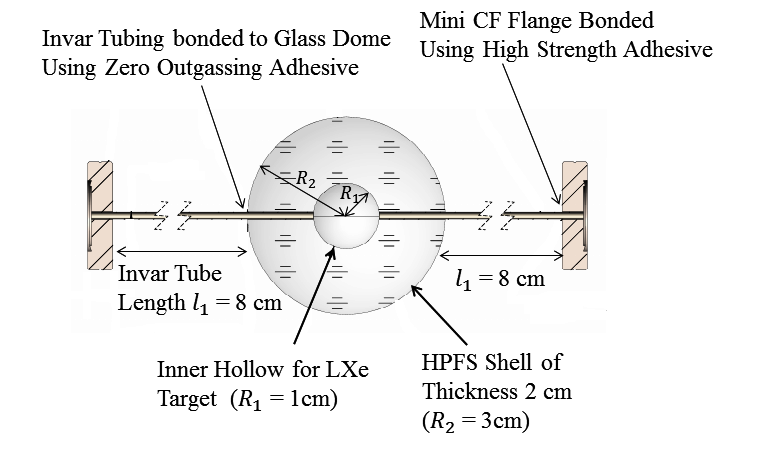
\includegraphics[width=\textwidth]{spheredesign1.png}
\end{subfigure}
\begin{subfigure}[c]{0.25\textheight}
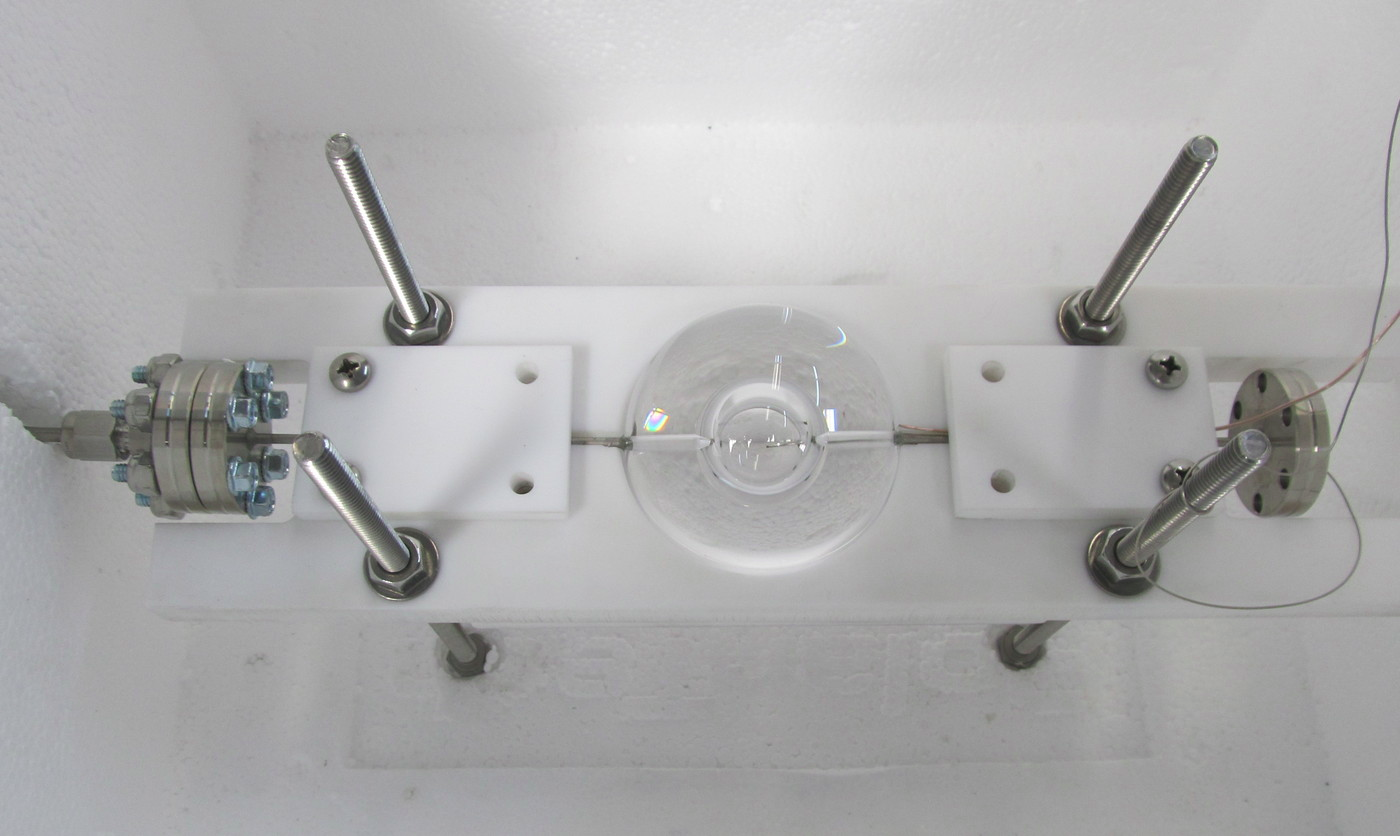
\includegraphics[width=\textwidth]{spherephoto.png}
\end{subfigure}
\caption{(Left)The technical design of the HPFS shell with Invar tubing and mini CF flanges. 
(Right) The industrially manufactured HPFS shell, held in a test fixture.} 
\label{fig:sphere}
\end{figure}
%%%%%%%%%%%%%%%%%%%%%%%%%%%%%%%%%%%%%%%%%%%%%%%%%%%%%%%%%%%%%%%%%%%%%%%%

%%%%%%%%%%%%%%%%%%%%%%%%%%%%%%%%%%%%%%%%%%%%%%%%%%%%%%%%%%%%%%%%%%%%%%%



Photons emitted from the LXe in the sphere are detected by 20  PMTs\footnote{R8520-406 Hamamatsu 1" PMT, active area 20.5 mm $\times 20.5 mm$}. 
The PMTs are chosen to have a quantum efficiency greater than 30\% at 178\,nm. The voltage applied on each PMT (the maximum is +900V) is adjusted such that the gain of the PMT is ~ 2 $\times$ 10$^6$. A positive voltage divider\footnote{Hamamatsu VDS18130p 24 channel positive polarity.} is used to to provide high voltage to the PMTs. 
The PMTs are held with a special aluminum holder, coated with anti-reflection color. 
The holder is made of two hemispheres hosting the PMTs in 3 rows, all of them pointing to the 
center of the sphere. The PMTs are attached to the holder by their voltage--divider bases using M2 PEEK screws (see Fig~\ref{fig:pmtholder}). 
The CAD design and a photo of the detector system are shown 
in Fig.~\ref{fig:detector}.

%%%%%%%%%%%%%%%%%%%%%%%%%%%%%%%%%%%%%%%%%%%%%%%%%%%%%%%%%%%%%%%%%%%%%%%%%%%%%%%%%%%%%%%%%%%
\begin{figure}[h]
   \centering
   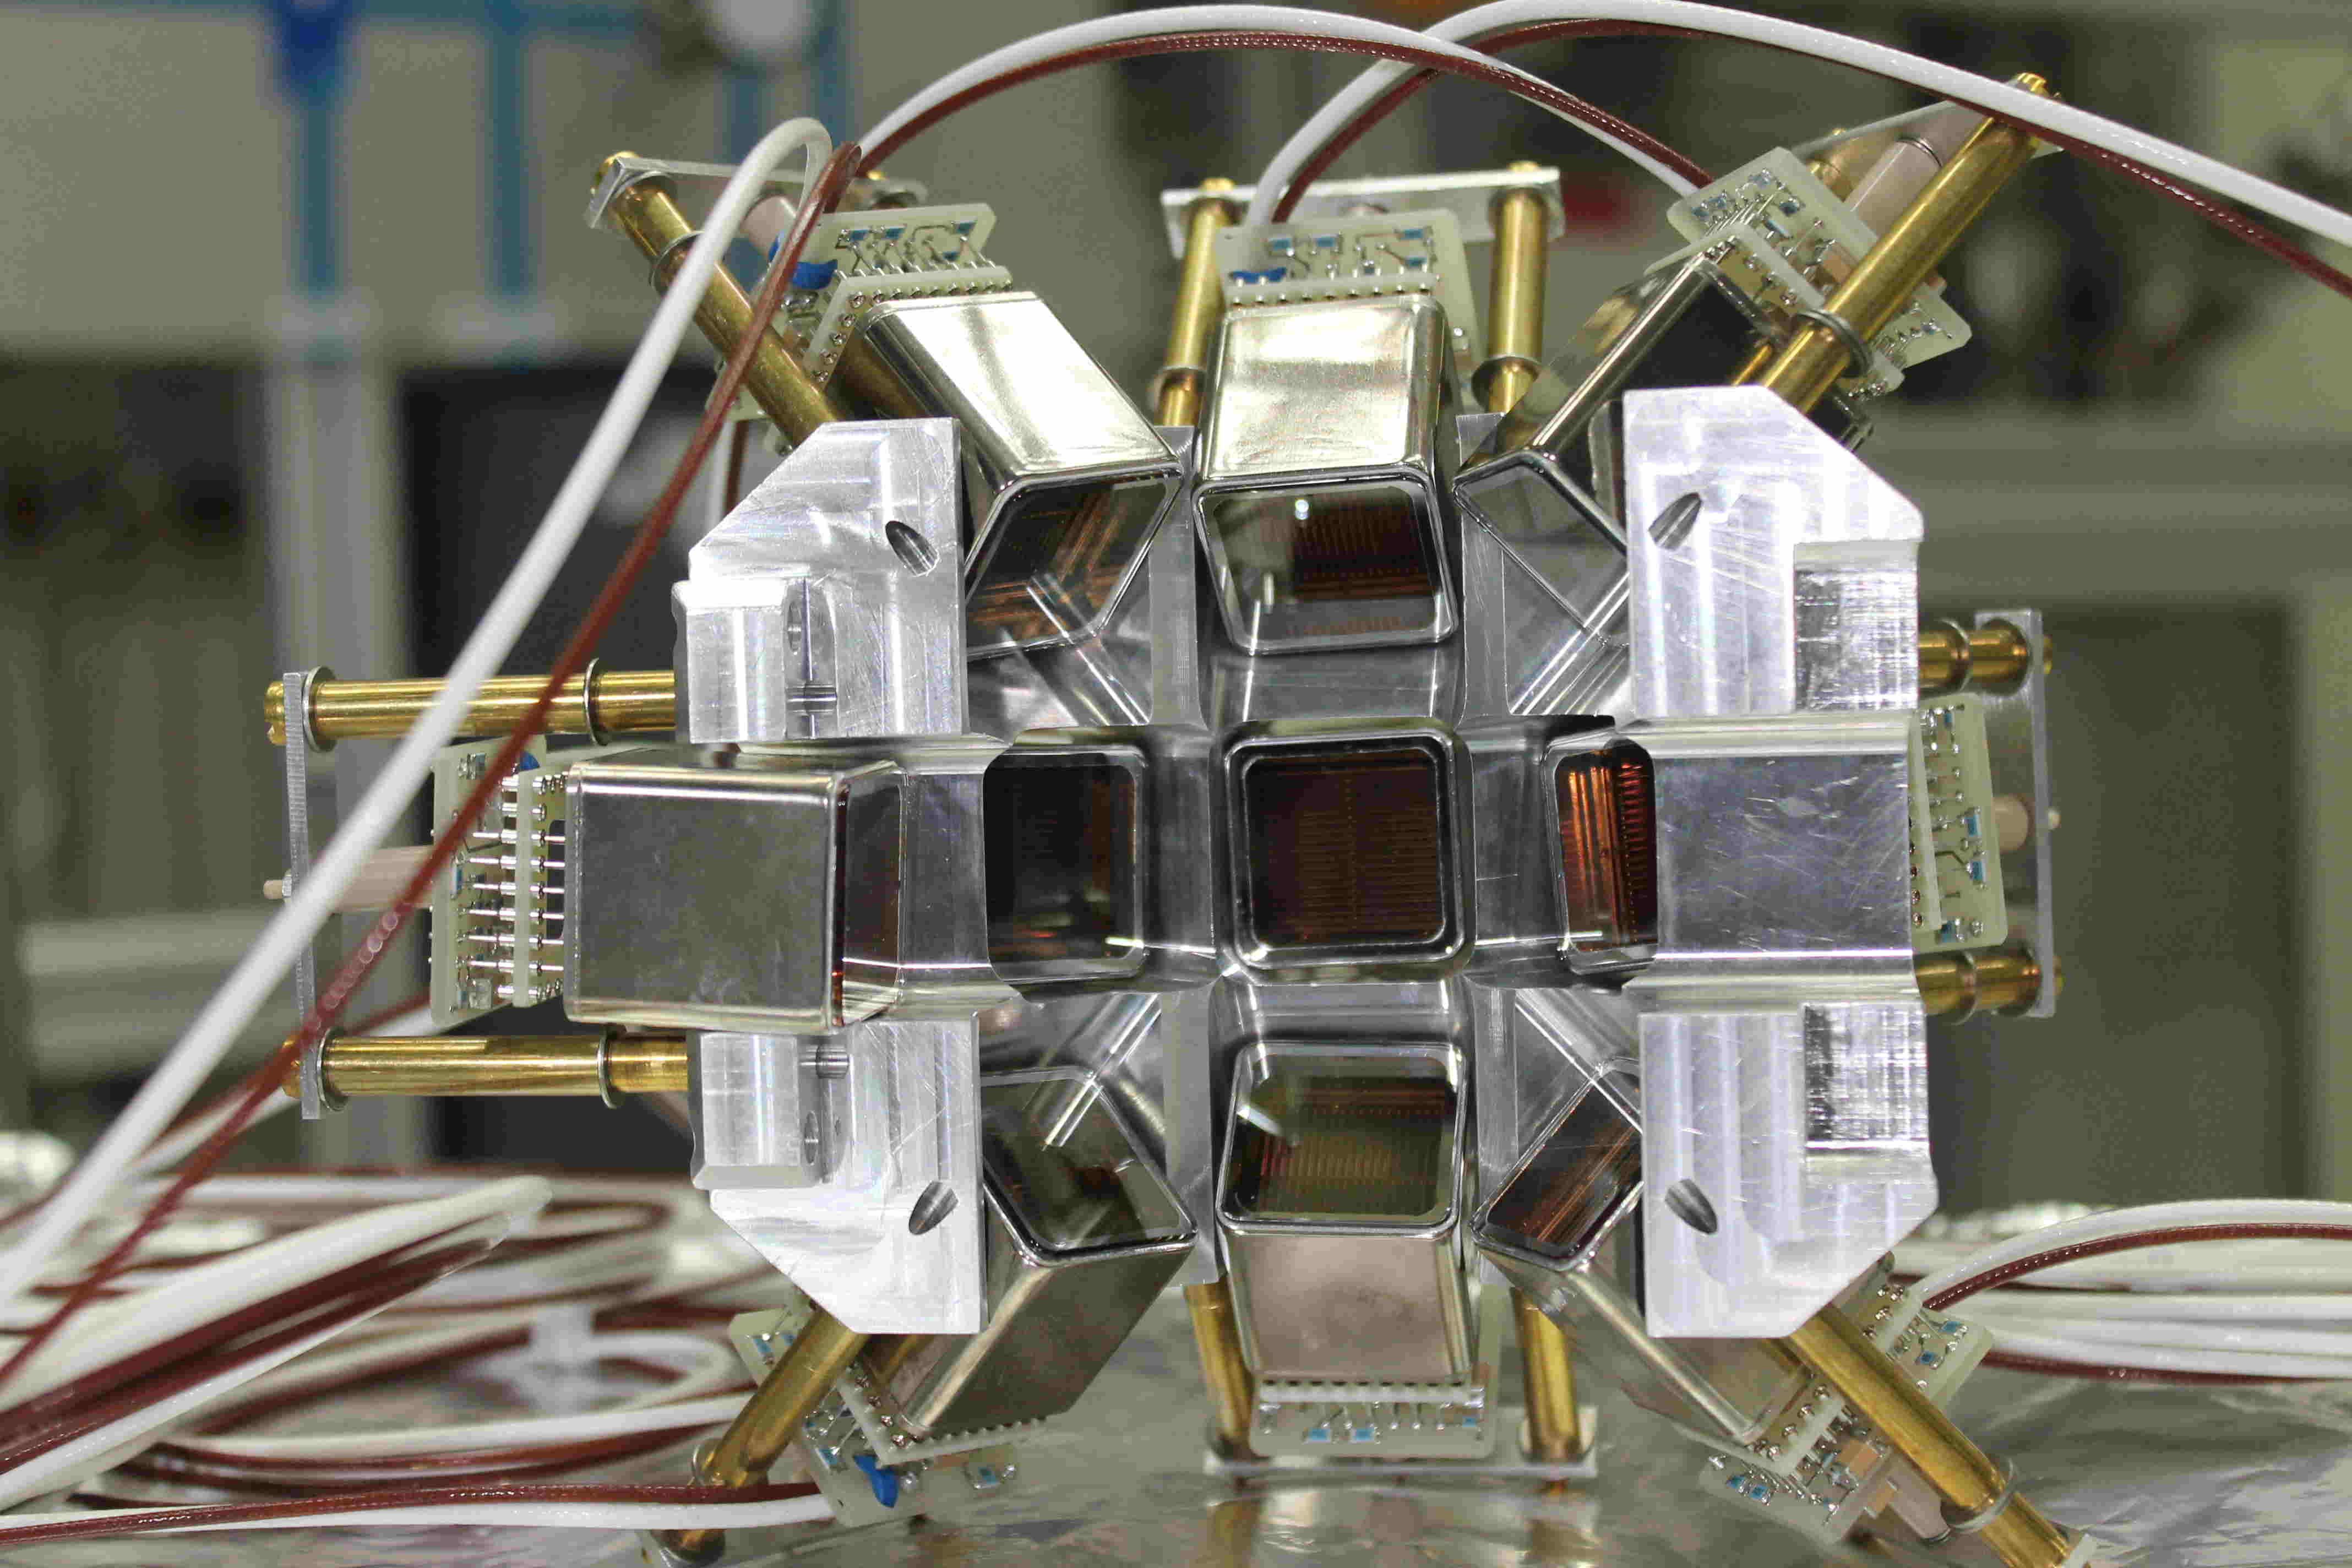
\includegraphics[width=0.5\textwidth]{PMTholder.JPG}
   \caption{A PMT holder--hemisphere. Two identical hemispheres are used to hold the PMTS around the sphere.} 
   \label{fig:pmtholder}
\end{figure}
%%%%%%%%%%%%%%%%%%%%%%%%%%%%%%%%%%%%%%%%%%%%%%%%%%%%%%%%%%%%%%%%%%%%%%%%%%%%%%%%%%%%%%%%%%%

%%%%%%%%%%%%%%%%%%%%%%%%%%%%%%%%%%%%%%%%%%%%%%%%%%%%%%%%%%%%%%%%%%%%%%%%%%
\begin{figure}[h]
\centering
\begin{subfigure}[c]{0.45\textwidth}
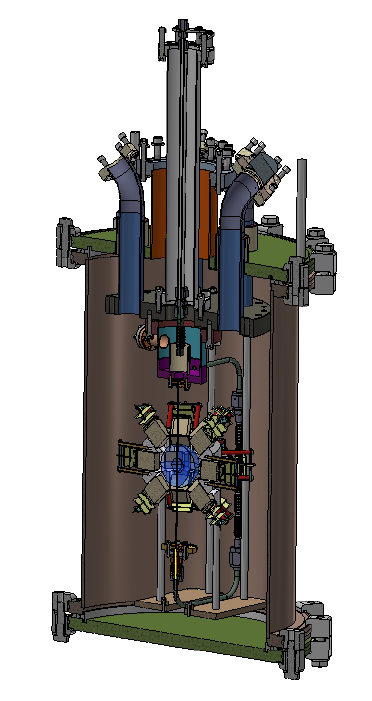
\includegraphics[width=0.75\textwidth , height=0.3\textheight]{detCAD.png}% Here is how to import 
\end{subfigure}	
\begin{subfigure}[c]{0.45\textwidth}
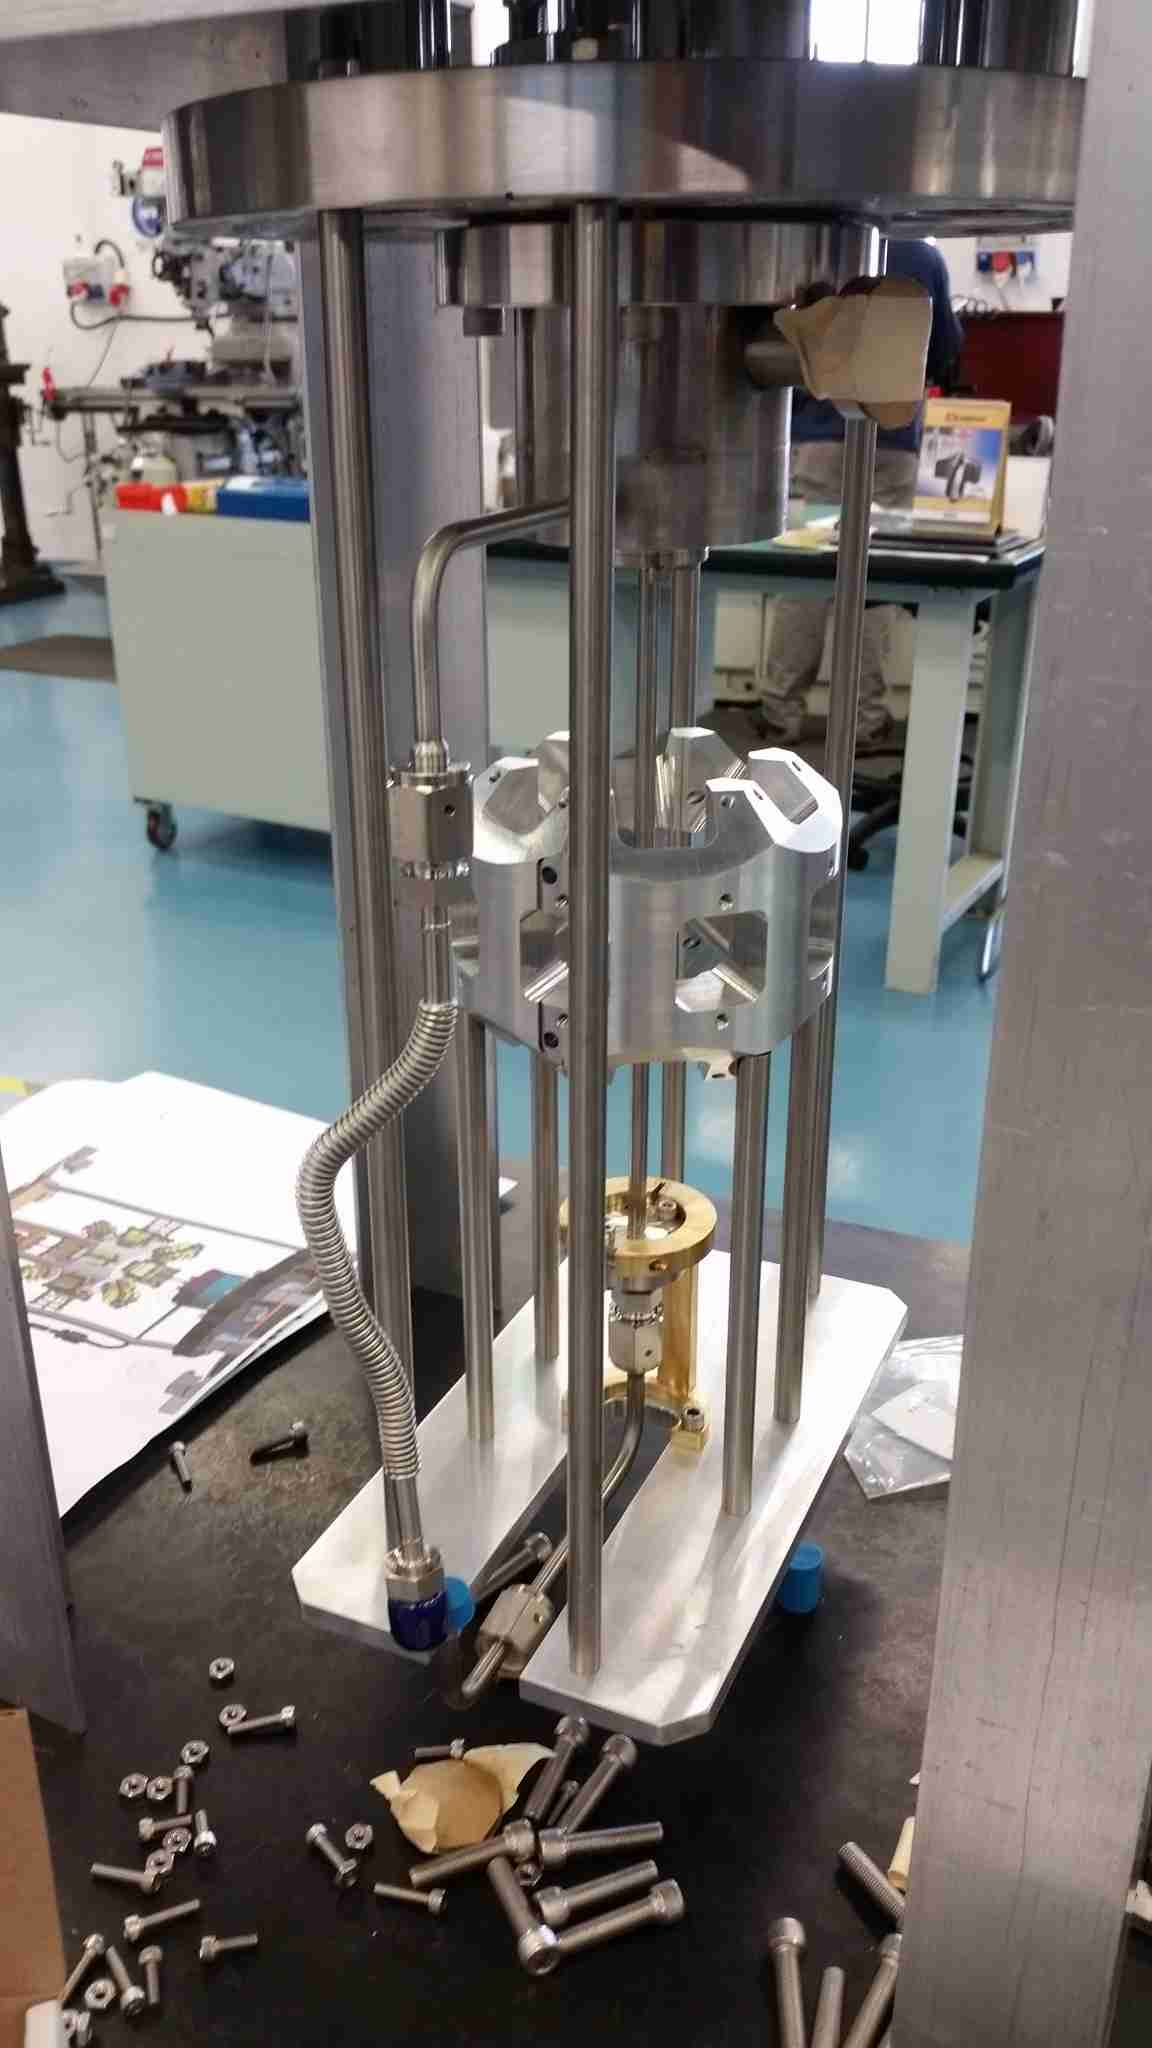
\includegraphics[width=\textwidth , height=0.3\textheight]{detReal_small.jpg}% Here is how to import 
\end{subfigure}	
\caption{\label{fig:detector} (Left) CAD design of the detector part. (Right) First mounting of the 
detector part, still not connected to the rest of the system.}
\end{figure}
